\section{Resilience}

In this section, we present the fault tolerance mechanism and flow migration protocol used by NFActor framework. Before going into the details, we first compare the difference between 

\subsection{Fault Tolerance}
\label{sec:ft}

In this section, we introduce the fault tolerance mechanisms for our NFActor
framework, including the controller, the virtual switch, and the runtimes. 
Depending on the nature of these three components, we carefully design 
lightweight fault-tolerance mechanisms for them so that these mechanisms be 
robust and have little performance impact in normal case.

\subsubsection{Replicating Controller}

Since the controller is a singled-threaded server that stores the states of 
the NFActor runtime, we persistently log these states and replicate them. The 
controller only needs to log the state of each NFActor runtime in 
the cluster view list. Whenever the controller needs to modify the state of a 
runtime, it logs the intended operation, modifies the state and logs a success 
mark for the intended operation.

The liveness of the controller is monitored by a guard process and the 
controller is restarted immediately in case of failure. On a reboot, the 
controller reconstructs the state in the cluster view list by replaying log. 
Each runtime in the cluster monitors the connection status with the controller 
and reconnects to the controller in case of a connection failure.

\subsubsection{Replicating Virtual Switch}

The most important state of the virtual switch process is its switching hash 
table in memory. In order to replicate the virtual switch, we constantly 
check-point the container memory image of the virtual switch using CRIU 
\cite{criu}, a popular tool for checkpoint/restore Linux processes. One main 
technical challenge is that CRIU has to stop a process before checkpointing it, 
which may hurt the availability of the virtual switch.

We tackle this challenge by letting the virtual switch call a 
fork() periodically (by default, one minute), and then we use CRIU to checkpoint 
the child process. Therefore, the virtual switch can proceed without affecting 
NFActor performance.

% Since the
% check-pointing needs to halt the execution of the whole virtual switch, it can
% not be frequently performed. In our implementation, we create a check-point for
% every second. However, this means that some states in the switching hash table
% might be lost and the flow connection related with these states may be forced to
% terminate. We argue that this is an acceptable implementation trade-off as flows
% could do a reconnection to complete unfinished tasks. If strong consistency is
% required, the virtual switch could use the replication strategy of
% FTMB\cite{sherry2015rollback}, we leave this to the future work.

\subsubsection{Replicating Runtime}

\begin{figure}
	\begin{subfigure}[b]{0.45\columnwidth}
		\centering
		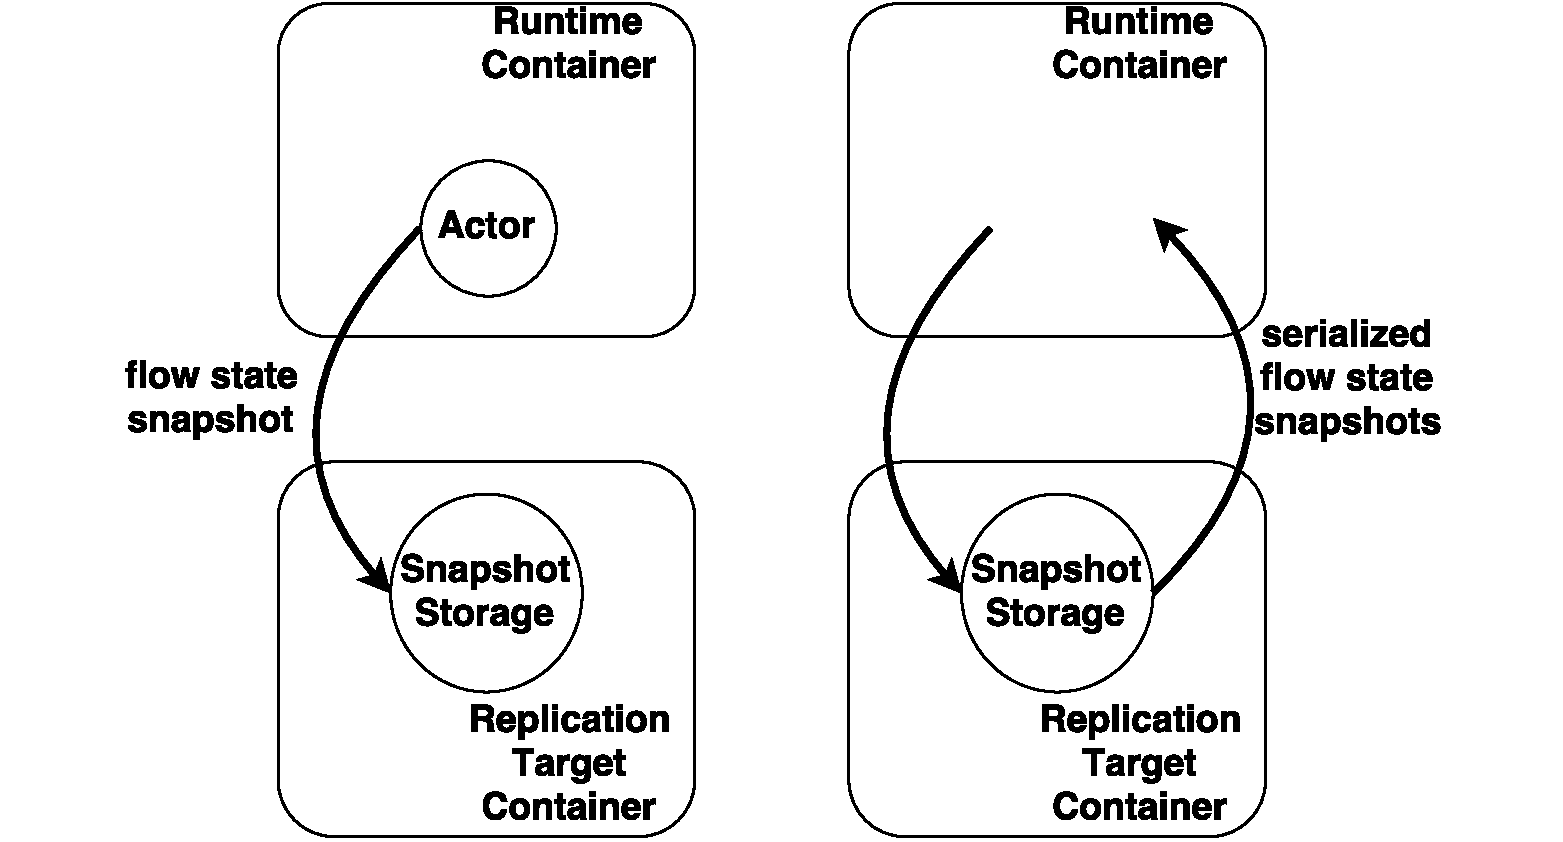
\includegraphics[width=\columnwidth]{figure/NFActor-Runtime-Replicate.pdf}
		\caption{Actor replicates its flow state to another
		runtime.}\label{fig:replicate} \end{subfigure}\hfill
	\begin{subfigure}[b]{0.45\columnwidth}
		\centering
		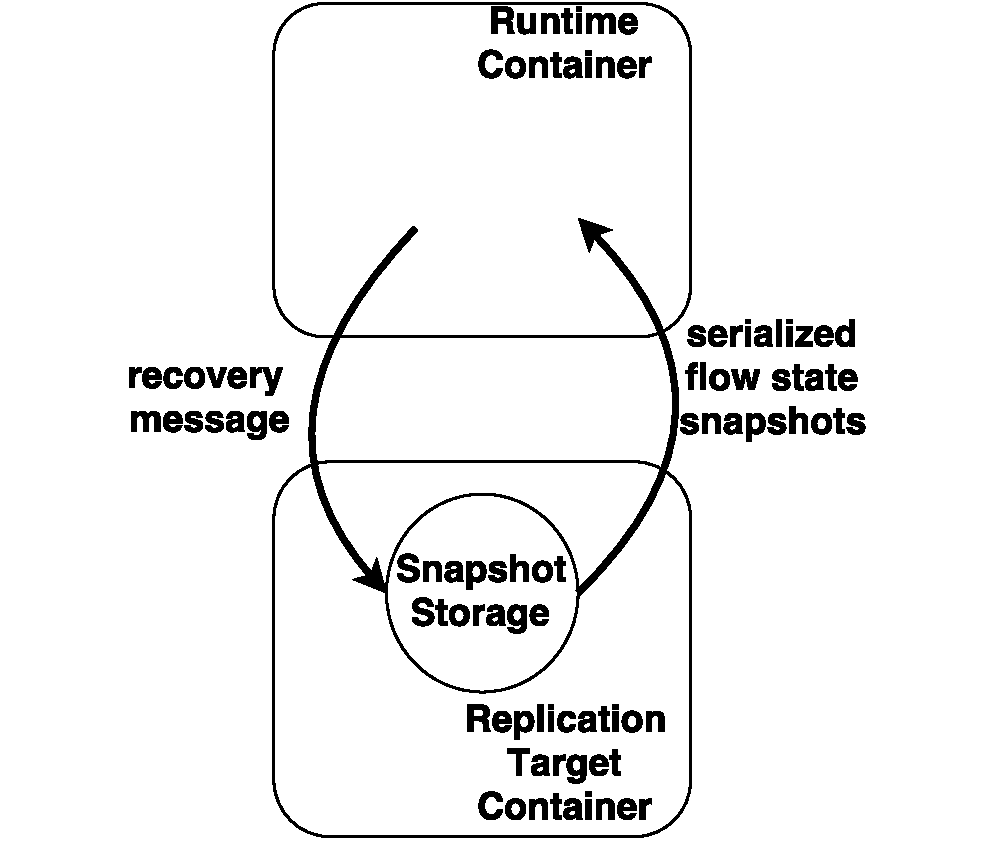
\includegraphics[width=\columnwidth]{figure/NFActor-Runtime-Recover.pdf}
		\caption{A failed runtime is restarted.}\label{fig:recover}
	\end{subfigure}%
\caption{Replication strategy for NFActor runtime.}
\end{figure}

To perform lightweight NFActor runtime replication, we leverage the actor 
abstraction and state separation to create a lightweight flow state replication 
strategy. In NFActor runtime, important flow states associated with a flow is 
owned by a unique actor. NFActor runtime can replicate each actor 
independently without incurring the overhead of check-pointing the entire 
container images \cite{sherry2015rollback, rajagopalan2013pico}.

This primary-backup replication manner can tolerate one actor failure at 
runtime, and we think this fault-tolerance guarantee is sufficient because the 
chance two actor machines failing at the same time is extremely rare.

\textbf{Find A Replication Target}: When the actor is created, it selects a
\textit{running} state runtime with the smallest workload as its replication
target. Then the actor negotiates with the replication target about whether the
replication target can accept this actor's replica. In case that replication
target refuses to store the actor's replica, the actor tries to select
another replication target. 

\textbf{Flow State Replication (figure \ref{fig:replicate})}: After determining
the replication target, the actor performs flow state replication. Before the input packet is processed on
the service chain, the actor saves a copy of the input packet. After the packet
finishes being processed on the service chain, the actor sends the local runtime
ID, flow identifier, original input packet and the processed packet to the
replication target. For every fixed number of packets that the actor has processed, the actor create a
snapshot of all the flow states and send the snapshot to the replication target as well.

When the replication target receives a new replication message, it saves the
message content in the RAM. If received message includes a new state snapshot,
replication target wipes out all previously saved content associated with the flow and save the new
state snapshot as well. Then the replication target sends the processed
packet out from its output port to the virtual switch. The flow state
replication procedure ensures the same output commit property as indicated in
\cite{sherry2015rollback}.

\textbf{Recover Failed Runtime (figure \ref{fig:recover})}: If a NFActor runtime
fails, it's failure will be detected by the controller after a timeout. Then the failed NFActor runtime will be restarted
with the same runtime ID. The restarted NFActor then starts recovery process. It
sends to all the other NFActor runtimes in the cluster a recover message, which
contain its NFActor runtime id. Other NFActor runtimes respond to the recover
message by sending all the replicas with the same runtime ID back to the
restarted NFActor runtime. The restart NFActor runtime then use these replicas
to reconstruct its state before failure. When the NFActor runtime finishes
recovery, it sends a {\tt join} message back to the controller to re-join the
cluster. 

% \textbf{Discussion}: The runtime replication strategy can tolerate at most one
% failed runtime. If multiple runtimes fail concurrently, then the replicas will
% be lost and the states of some flows will never be correctly recovered.
% Multi-machine replication algorithm such as PAXOS \cite{chandra2007paxos} could
% be used to replicate the flow state to multiple backups. However, PAXOS may not
% be efficient enough to handle the replication of a large number of packets. We
% leave exploring multi-backup to our future work. 

%%%%%%%%%%%%%%%%%%%%%%%%%%%The following is flow migration%%%%%%%%%%%%%%%%%%%%%%%%%

\subsection{Distributed Flow Migration}
\label{sec:fm}

In this section, we present the distributed flow migration method of NFActor
framework. There are some problems with existing flow migration
framework \cite{gember2015opennf, rajagopalan2013split}. First they all use a
centralized controlelr to monitor the entire flow migration
process. This is not scalable. The second problem is that the flow migration
protocol is too complicated to implement. Patch code needs to be added to the
core processing logic of the NFs. The flow migration protocol needs to exchange
multiple messages among controller, switches and NF instances. This increases
the possibility of serious software bugs. The final problem is that the NF can
not start the flow migration process by itself. It must be started from the
controller. This stops the NFs from making timely responses to overload signal.

All the above mentioned problems could be solved using NFActor framework. In
NFActor framework, the NF packet processing is carried out within the
execution context of the actor. This additional layer of monitoring gives
NFActor power to start flow migration from the NFActor runtime. On the other
hand, the API design forces a clean separation between flow state and NF
processing logic, making extracting and serializing flow state an easy task.
NFActor framework also has a built-in message-passing functionality that
makes flow migration simpler. In this section, we elaborate in detail how flow
migration works in NFActor framework.

\subsubsection{Distributed Flow Migration Protocol}

\begin{figure*}[!t]
	\begin{subfigure}[t]{0.23\linewidth}
		\centering
		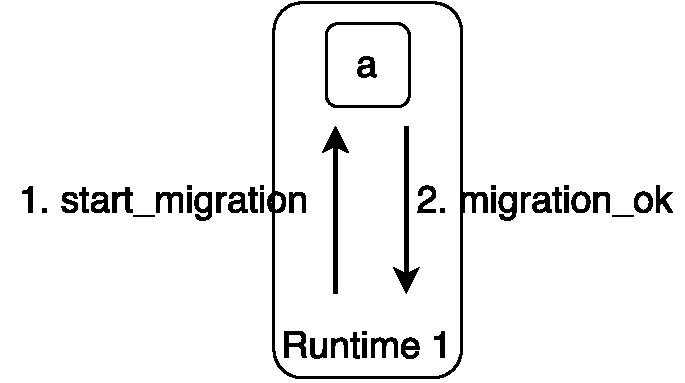
\includegraphics[width=\columnwidth]{figure/NFActor-Flow-Migration-Init.pdf}
		\caption{Initiate flow migration.}\label{fig:init} 
	\end{subfigure}\hfill
	\begin{subfigure}[t]{0.23\linewidth}
		\centering
		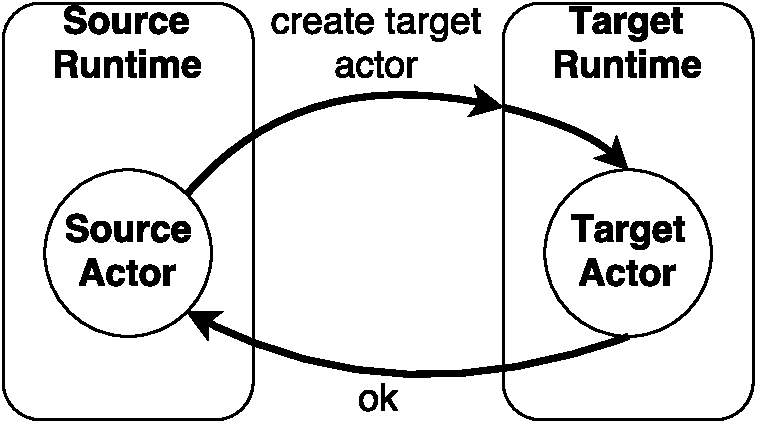
\includegraphics[width=\columnwidth]{figure/NFActor-Flow-Migration-First.pdf}
		\caption{Create target actor.}\label{fig:first} \end{subfigure}\hfill
	\begin{subfigure}[t]{0.23\linewidth}
		\centering
		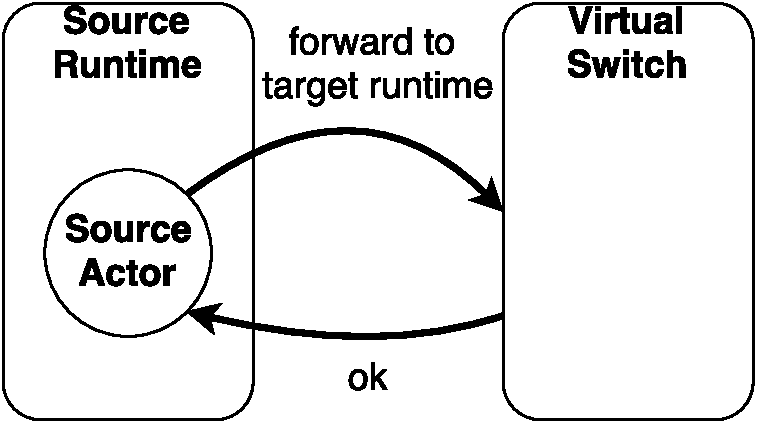
\includegraphics[width=\columnwidth]{figure/NFActor-Flow-Migration-Second.pdf}
		\caption{Contact virtual switch.}\label{fig:second}
	 \end{subfigure}\hfill
	 \begin{subfigure}[t]{0.23\linewidth}
		\centering
		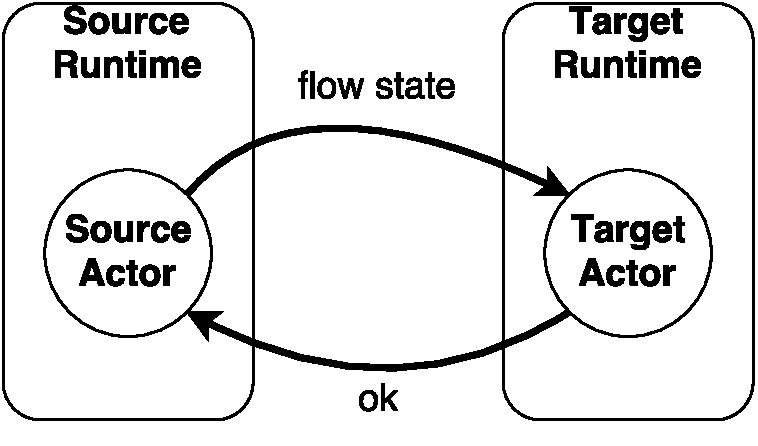
\includegraphics[width=\columnwidth]{figure/NFActor-Flow-Migration-Third.pdf}
		\caption{Migrate flow state.}\label{fig:third}
	 \end{subfigure}
\caption{Distributed Flow Migration Protocol of NFActor Framework}
\label{fig:migration}
\end{figure*}

The distributed flow migration protocol is shown in figure \ref{fig:migration}.
It consists of passing 4 request-response. We first show successful
request-response in figure \ref{fig:migration} and then supplement possible
failure cases.

\textbf{Initiate Flow Migration}: As shown in figure \ref{fig:init}, the flow
migration in NFActor is initiatied by sending a {\tt start\_migration} message
from the NFActor runtime 1 to an actor \textit{a} on this runtime. The {\tt
start\_migration} message contains a ID of a target runtime. Runtime 1 acquires
this ID by querying the view service. Once actor \textit{a} receives this
message, it starts the migration process by itself, without involving a centralized controller.

Runtime 1 is promised to receive a response from actor \textit{a}. A {\tt
migration\_ok} message sent from actor \textit{a} indicates that the migration
is successfully finished. The flow being migrated has
resumed its execution on the target runtime. Actor \textit{a} has quit
execution and released all its resources. The migration can of course fail due
to many reasons. In that case, actor \textit{a} will respond a {\tt
migration\_fail} message back to runtime 1 and continue to process flow packets
on runtime 1.

\textbf{Create Target Actor:} Actor \textit{a} then sends a {\tt create\_target\_actor} request message to the
target runtime 2, expecting a response. This message also contains the flow
identifier of actor \textit{a}. Target runtime 2 target runtime 2 creates a target
actor \textit{b}, registers target actor \textit{b} using the flow identifer
contained in the {\tt start\_migration} message and delegates the migration
process to target actor \textit{b}. Target actor \textit{b} then responds a {\tt
ok} message to actor \textit{a}.

\textbf{Contact Virtual Switch:} Actor \textit{a} sends a {\tt
forward\_to\_target\_runtime} request message to the virtual switch. This
message contains the flow identifier and the ID of the target runtime 2. After
virtual switch has received the request message, the virtual switch first
updates its switching hash table by changing the value associated with the flow identifier
to the ID of target runtime 2. Then the virtual switch creates a data-plane
packet with the same flow identifier contained in the message and fills the
payload with a global unique magic-number. Then the virtual switch sends this
data-plane packet back to runtime 1.

When actor \textit{a} receives the data-plane packet with the magic number, it
knows that the no more flow packets will be forwarded to itself. Then actor
\textit{a} can safely migrate its flow state to the target actor \textit{b}. The
use of the data-plane packet instead of control message ensures lossless flow
migration \cite{gember2015opennf}. In case that actor \textit{a} fails to
receive data-plane response packet after a timeout, actor \textit{a} will
re-send {\tt forward\_to\_target\_runtime} to the virtual switch.

After virtual switch updates its switching hash table, target actor \textit{b}
starts to receive flow packets. Target actor \textit{b} only buffers these
packets and waits until flow state migration complete before processing them.

\textbf{Migrate Flow State:} Actor \textit{a} sends a {\tt migrate\_flow\_state}
request message, along with the serialized flow states of actor \textit{a}, to
target actor \textit{b}. After receving the request message, target actor
\textit{b} first responds a {\tt ok} message back to actor \textit{a}.
Then it drains all the buffered packets and resumes normal flow packet
processing. 

Actor \textit{a} on the other hand, waits until it receives {\tt ok} message
from target actor \textit{b}. Then it responds a {\tt migration\_ok} message
back to runtime 1, destroies all the of its resources and quits.

\subsubsection{Failure Handling}
 
The flow migration protocol in figure \ref{fig:first} to \ref{fig:third} may
generate different kinds of failures. This causes actor \textit{a} in figure
\ref{fig:init} to responds a {\tt migration\_fail} message back to runtime 1. In
this section, we analyze possible failures and how to handle these failures.
Flow migration protocol relies on failure recovery to handle some serious
failures. For the flow migration process, the target actor does not maintain a
replica. In the meantime, the actor being migrated does not log that it is being
migrated. This means that if the runtime involved in the migration fails, the
migration is implicitly stopped.

\textbf{Target runtime is overloaded.} In figure \ref{fig:first},
when target runtime 2 receives {\tt create\_target\_actor} message, it first
checks whether it is overloaded before creating target actor \textit{b}.
This is because runtime 1 uses the view service to determine target runtime and
the view service is not an always-up-to-date service. Target runtime 1 may
experience overload and it can not accept new migrated actors. In that case,
target runtime 2 respond a {\tt fail} response back to actor \textit{a}, causing
actor \textit{a} to stop the migration.

\textbf{Messages are lost in the network.} In figure \ref{fig:first}, if either
the {\tt create\_target\_actor} message or the response message is lost, actor
\textit{a} stops migration. This also causes a timeout to be triggered on target
actor \textit{b} and stops \textit{b}. Figure \ref{fig:second} and
\ref{fig:third} involve changing packet forwading path and migrating flow state.
The migration can not be simply stopped due to message loss. In figure
\ref{fig:second}, actor \textit{a} just keeps re-sending the request message
until it receives a definitive response. In figure \ref{fig:third}, actor
\textit{a} keep retrying for a fixed number of times. Then it performs a live
recovery.

\textbf{Runtime fails.} In figure \ref{fig:first}, the failure of either runtime
simply halts the migration process. In figure \ref{fig:second} and
\ref{fig:third}, actor \textit{a} and target actor \textit{b} monitor each
other. The failure of runtime 1 causes target actor \textit{b} not to receive
{\tt migrate\_flow\_state} message. Actor \textit{b} requests the virtual switch
to forward to runtime 1. The failure of target runtime 2 causes actor \textit{a}
to perform a live recovery. 

\textbf{Buffer Overloads.} After virtual switch updates its switching hash
table, target actor \textit{b} starts to buffer the packets. We set a maximum
capacity for the buffer. If the buffer is full when receiving {\tt
migrate\_flow\_state} message, target actor \textit{b} responds a {\tt fail}
message to actor \textit{a}, causing \textit{a} to perform a live recovery.

\textbf{Virtual Switch Fails.} After virtual switch is restarted, it may lost
some states in the switching hash table. The flow being migrated may be forced
to terminate due to inconsistent state.









